% atifcppprogrammers's Data Communication Lab Report Template.%
\documentclass[fullpage]{article}
\usepackage{tgpagella}
\usepackage{graphicx}
\usepackage{float}
\usepackage[english]{babel}
\usepackage[latin1]{inputenc}

\begin{document}

   \title{Experiment 3 - Simple Topology in NS-3}

   \author{Muhammad Atif Farooq L144392 EL-A}

   \date{14th Septemeber 2019}

   \maketitle

\section{Introduction}
Whenever data is transferred over a computer network, the packets constituing that
data travel through what are know as \textbf{Routers}. These routers read the
destination IP on these packets and use the routing tables to determine the most
efficient course for the packet to travel to reach its destination. It is this
phenomenon of \textbf{Routing} which we aim to explore in this experiment.

\section{Objective}
Build and analyze a small point to point link in NS-3 using routing.

\section{Procedure}
We begin by briefly discussing the topology in question and then remark on our efforts to
realize the aforementioned topolgy in NS-3.

\subsection{The Topology}
As in the previous lab, we were required to set up a point to point link between the
client and server nodes, however in this iteration an additional stipulation demanded
the presence of an intermediary node acting as a router. The topology in question can be
summarized succintly by the following illustration.

\begin{figure}[H]
  
\includegraphics[width=\linewidth]{topologyLabQuestion.png}
  \caption{point to point link}
  \label{fig:output2}
\end{figure}

\subsection{Stratedgy Employed}
We begin by creating a single node container to house the three nodes required by
our topology, we then isolated the above three nodes into two node containers one
for the client and one for the server with the router being shared between them.
This was followed by the general NS-3 procedure of specifying the point to point link,
installing the network cards, protocol stacks and installing the client and server apps
on the appropriate nodes. Finally the line \verb|Ipv4GlobalRoutingHelper::PopulateRoutingTables()|
was included to allow routing of packets.

The code written to simulate the behaviour of the above topology, in addition to the
console output is presented below.

\begin{verbatim}
  #include "ns3/core-module.h"
  #include "ns3/network-module.h"
  #include "ns3/internet-module.h"
  #include "ns3/point-to-point-module.h"
  #include "ns3/applications-module.h"

  using namespace ns3;

  NS_LOG_COMPONENT_DEFINE ("FirstScriptExample");

  int
  main (int argc, char *argv[])
  {
    CommandLine cmd;
    cmd.Parse (argc, argv);

    Time::SetResolution (Time::NS);
    LogComponentEnable ("UdpEchoClientApplication", LOG_LEVEL_INFO);
    LogComponentEnable ("UdpEchoServerApplication", LOG_LEVEL_INFO);

    // Creating Three Nodes Required by Topology.
    NodeContainer allNodes;
    allNodes.Create(3);

    // Node Container for Client and Router.
    NodeContainer clientRouterNodes = NodeContainer(allNodes.Get(0),
      allNodes.Get(1));

    // Node Container for Server and Router.
    NodeContainer routerServerNodes = NodeContainer(allNodes.Get(1),
      allNodes.Get(2));

    // Specifying Point to Point Link Between Client and Router.
    PointToPointHelper pointToPointOne;
    pointToPointOne.SetDeviceAttribute("DataRate",StringValue("5Mbps"));
    pointToPointOne.SetChannelAttribute("Delay",StringValue("2ms"));

    // Specifying Point to Point Link Between Server and Router.
    PointToPointHelper pointToPointTwo;
    pointToPointTwo.SetDeviceAttribute("DataRate",StringValue("5Mbps"));
    pointToPointTwo.SetChannelAttribute("Delay",StringValue("2ms"));

    // Installing Net-Devices for Client Rotuer Link.
    NetDeviceContainer devicesOne;
    devicesOne = pointToPointOne.Install(clientRouterNodes);

    // Installing Net-Devices for Server Router Link.
    NetDeviceContainer devicesTwo;
    devicesTwo = pointToPointTwo.Install(routerServerNodes);

    // Installing Protocol Stack on Client and Router.
    InternetStackHelper stackOne;
    stackOne.Install(clientRouterNodes);

    // Installing Protocol Stack on Server.
    InternetStackHelper stackTwo;
    stackTwo.Install(routerServerNodes.Get(1));

    // Setting Address for Client Router Link.
    Ipv4AddressHelper addressOne;
    addressOne.SetBase ("192.168.40.0", "255.255.255.0","0.0.0.1");

    Ipv4InterfaceContainer interfacesOne = addressOne.Assign (devicesOne);

    // Setting Address for Server Router Link.
    Ipv4AddressHelper addressTwo;
    addressTwo.SetBase ("192.168.41.0", "255.255.255.0","0.0.0.1");

    Ipv4InterfaceContainer interfacesTwo = addressTwo.Assign (devicesTwo);

    // Installing Server-Apps.
    UdpEchoServerHelper echoServer (9);

    ApplicationContainer serverApps = echoServer.Install (routerServerNodes.Get(1));
    serverApps.Start (Seconds (1.0));
    serverApps.Stop (Seconds (10.0));

    // Installing Client-Apps.
    UdpEchoClientHelper echoClient (interfacesTwo.GetAddress (1), 9);
    echoClient.SetAttribute ("MaxPackets", UintegerValue (6));
    echoClient.SetAttribute ("Interval", TimeValue (Seconds (1.0)));
    echoClient.SetAttribute ("PacketSize", UintegerValue (1024));

    ApplicationContainer clientApps = echoClient.Install (clientRouterNodes.Get (0));
    clientApps.Start (Seconds (2.0));
    clientApps.Stop (Seconds (10.0));

    // To Enable Routing.
    Ipv4GlobalRoutingHelper::PopulateRoutingTables();

    Simulator::Run ();
    Simulator::Destroy ();
    return 0;
  }
\end{verbatim}

\begin{figure}[H]
  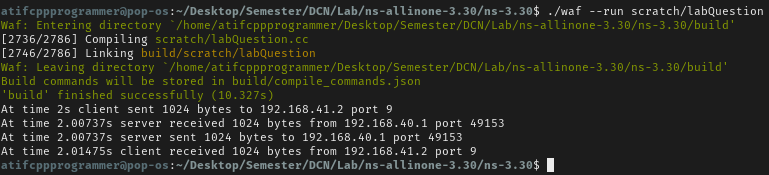
\includegraphics[width=\linewidth]{labQuestion.png}
  \caption{labQuestion.cc}
  \label{fig:output2}
\end{figure}

\section{Conclusions}
NS-3 allows us to simulate the behaviour of computer networks in particular
enabling us to model the process of routing packets over a network.

\section{Post-Lab Question}
For the post lab question we were required to implement the topology illustrated below
in NS-3.

\begin{figure}[H]
  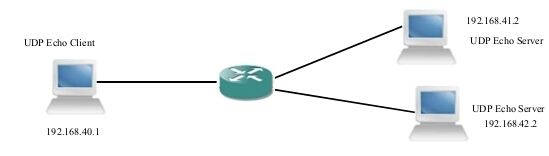
\includegraphics[width=\linewidth]{topologyPostLabQuestion.png}
  \caption{A more complex topology}
  \label{fig:output2}
\end{figure}

The required code and the accompanying console output is presented below.

\begin{verbatim}
  #include "ns3/core-module.h"
  #include "ns3/network-module.h"
  #include "ns3/internet-module.h"
  #include "ns3/point-to-point-module.h"
  #include "ns3/applications-module.h"

  using namespace ns3;

  NS_LOG_COMPONENT_DEFINE ("atifcppprogrammer_post_lab");

  int
  main (int argc, char *argv[])
  {
    CommandLine cmd;
    cmd.Parse (argc, argv);

    Time::SetResolution (Time::NS);
    LogComponentEnable ("UdpEchoClientApplication", LOG_LEVEL_INFO);
    LogComponentEnable ("UdpEchoServerApplication", LOG_LEVEL_INFO);

    // Creating all nodes required by topology.
    NodeContainer allNodes;
    allNodes.Create(4);

    // Creating node container for client and router point to point link.
    NodeContainer clientRouterNodes;
    clientRouterNodes = NodeContainer(allNodes.Get(0),allNodes.Get(1));

    // Creating node container for router and first server.
    NodeContainer routerServerNodesOne;
    routerServerNodesOne = NodeContainer(allNodes.Get(1),allNodes.Get(2));

    // Creating node container for router and second server.
    NodeContainer routerServerNodesTwo;
    routerServerNodesTwo = NodeContainer(allNodes.Get(1),allNodes.Get(3));

    // Specifying point to point link between client and router nodes.
    PointToPointHelper pointToPoint;
    pointToPoint.SetDeviceAttribute("DataRate",StringValue("Mbps"));
    pointToPoint.SetChannelAttribute("Delay",StringValue("2ms"));

    // Specifying point to point link between router and first server.
    PointToPointHelper pointToPointOne;
    pointToPointOne.SetDeviceAttribute("DataRate",StringValue("Mbps"));
    pointToPointOne.SetChannelAttribute("Delay",StringValue("2ms"));

    // Specifying point to point link between router and second server.
    PointToPointHelper pointToPointTwo;
    pointToPointTwo.SetDeviceAttribute("DataRate",StringValue("Mbps"));
    pointToPointTwo.SetChannelAttribute("Delay",StringValue("2ms"));

    // Installing Network Cards on client router nodes.
    NetDeviceContainer devices;
    devices = pointToPoint.Install(clientRouterNodes);

    // Installing Network Cards on router and first server nodes.
    NetDeviceContainer devicesOne;
    devicesOne = pointToPointOne.Install(routerServerNodesOne);

    // Installing Network Cards on router and second server nodes.
    NetDeviceContainer devicesTwo;
    devicesTwo = pointToPointTwo.Install(routerServerNodesTwo);

    // Installing Protocol Stack on client router nodes.
    InternetStackHelper stack;
    stack.Install(clientRouterNodes);

    // Installing Protocol Stack on Servers.
    stack.Install(routerServerNodesOne.Get(1));
    stack.Install(routerServerNodesTwo.Get(1));

    // Assigning IP Addresses for client and router link.
    Ipv4AddressHelper address;
    address.SetBase ("192.168.40.0", "255.255.255.0");

    Ipv4InterfaceContainer interfaces = address.Assign (devices);

    // Assigning IP Addresses for router and first server nodes.
    address.SetBase ("192.168.41.0", "255.255.255.0");
    Ipv4InterfaceContainer interfacesOne = address.Assign (devicesOne);

    // Assigning IP Addresses for router and second server nodes.
    address.SetBase ("192.168.42.0", "255.255.255.0");
    Ipv4InterfaceContainer interfacesTwo = address.Assign (devicesTwo);

    // Creating server and installing Server Application on first Server.
    UdpEchoServerHelper echoServerOne(93);

    ApplicationContainer serverAppsOne = echoServerOne.Install(
        routerServerNodesOne.Get(1));
    serverAppsOne.Start (Seconds (1.0));
    serverAppsOne.Stop (Seconds (5.0));

    // Creating server and installing Server Application on second Server.
    UdpEchoServerHelper echoServerTwo(94);

    ApplicationContainer serverAppsTwo = echoServerTwo.Install(
        routerServerNodesTwo.Get(1));
    serverAppsTwo.Start (Seconds (5.0));
    serverAppsTwo.Stop (Seconds (10.0));

    // Creating and installing client application to communicate with first server.
    UdpEchoClientHelper echoClient (interfacesOne.GetAddress (1), 93);
    echoClient.SetAttribute ("MaxPackets", UintegerValue (1));
    echoClient.SetAttribute ("Interval", TimeValue (Seconds (1.0)));
    echoClient.SetAttribute ("PacketSize", UintegerValue (1024));

    ApplicationContainer clientAppsOne = echoClient.Install(
      clientRouterNodes.Get(0));
    clientAppsOne.Start (Seconds (2.0));
    clientAppsOne.Stop (Seconds (5.0));

    // Creating and installing client application to communicate with second server.
    echoClient = UdpEchoClientHelper(interfacesTwo.GetAddress (1), 94);
    echoClient.SetAttribute ("MaxPackets", UintegerValue (1));
    echoClient.SetAttribute ("Interval", TimeValue (Seconds (1.0)));
    echoClient.SetAttribute ("PacketSize", UintegerValue (1024));

    ApplicationContainer clientAppsTwo = echoClient.Install(clientRouterNodes.Get(0));
    clientAppsTwo.Start (Seconds (5.0));
    clientAppsTwo.Stop (Seconds (10.0));

    // To Enable Routing.
    Ipv4GlobalRoutingHelper::PopulateRoutingTables();

    Simulator::Run ();
    Simulator::Destroy ();
    return 0;
  }
\end{verbatim}

\begin{figure}[H]
  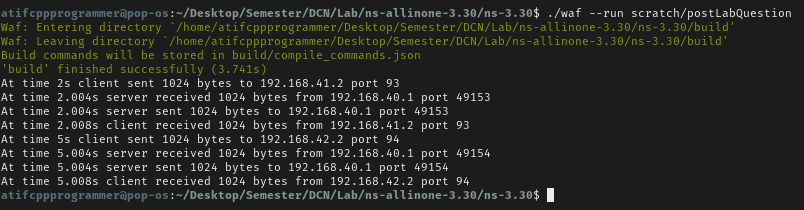
\includegraphics[width=\linewidth]{postLabQuestion.png}
  \caption{postLabQuestion.cc}
  \label{fig:output2}
\end{figure}

\end{document}
